\section*{Introducción}

Piensa en las ondas que se producen cuando una piedra cae en el agua, o en cómo se mueven las olas. Piensa en cómo la electricidad viaja a través de los cables (los cuales tienen forma de catenaria cuando se cuelgan, como bien sabes por artículos anteriores) y piensa en cómo el sonido se transmite por el aire hasta que llega a tu oído. Más aún, piensa en cómo la luz llega a tus ojos y en cómo las señales viajan rebotando entre satélites.

Puede que todavía no lo sepas, pero en todos esos casos aparecen las funciones periódicas, las cuales son tratadas bajo un marco que se conoce como \textit{Análisis de Fourier}. A lo largo y ancho de este artículo y otros subsiguientes iremos conociendo distintos aspectos de esta teoría, y si las cosas van bien, llegaremos a un punto en el que podremos apreciar la enorme influencia que ejerce en nuestras vidas.

En este primer artículo veremos la parte más teórica que usaremos en posteriores artículos con aplicaciones en circuitos eléctricos. El artículo presente está dividido como sigue: en la sección \ref{s:s1} estudiaremos lo que son las funciones periódicas y lo que son los armónicos; en la sección \ref{s:s2} daremos el teorema de representación de una función como suma de armónicos en su versión real y en la sección \ref{s:s3} haremos lo mismo pero desde el enfoque del campo complejo el cual reduce la teoría y permite una formulación más simple.


\section{Preliminares}\label{s:s1}
\subsection{Funciones periódicas}

La idea es intuitiva, pero necesitamos una definición rigurosa a la que atenernos.
\begin{mybox}
\textbf{Definición.} Consideremos una función $f:\mathbb{R}\longrightarrow\mathbb{R}$. Decimos que $f$ es \textbf{periódica} si existe algún número $T>0$ tal que:
\begin{equation} \label{eq:FuncionPeriodica}
f(x+T) = f(x) \qquad \forall x\in\mathbb{R} .
\end{equation}
Así, diremos que $T$ es un \textbf{período} de $f$. De entre todos ellos, el menor recibe el nombre de \textbf{período fundamental}.
\end{mybox}

Este concepto se puede visualizar muy fácilmente, ya que la ecuación \eqref{eq:FuncionPeriodica} significa que la gráfica se va repitiendo a intervalos de longitud $T$, como se ve en la Figura \ref{fig:FuncionPeriodica}.

\begin{figure}[h]
\begin{figurebox}
    \vspace{5pt}
    \centering
    \scalebox{0.4}{ % Title: glps_renderer figure
% Creator: GL2PS 1.3.8, (C) 1999-2012 C. Geuzaine
% For: Octave
% CreationDate: Mon Aug 11 13:59:37 2014
\setlength{\unitlength}{1pt}
\begin{picture}(0,0)
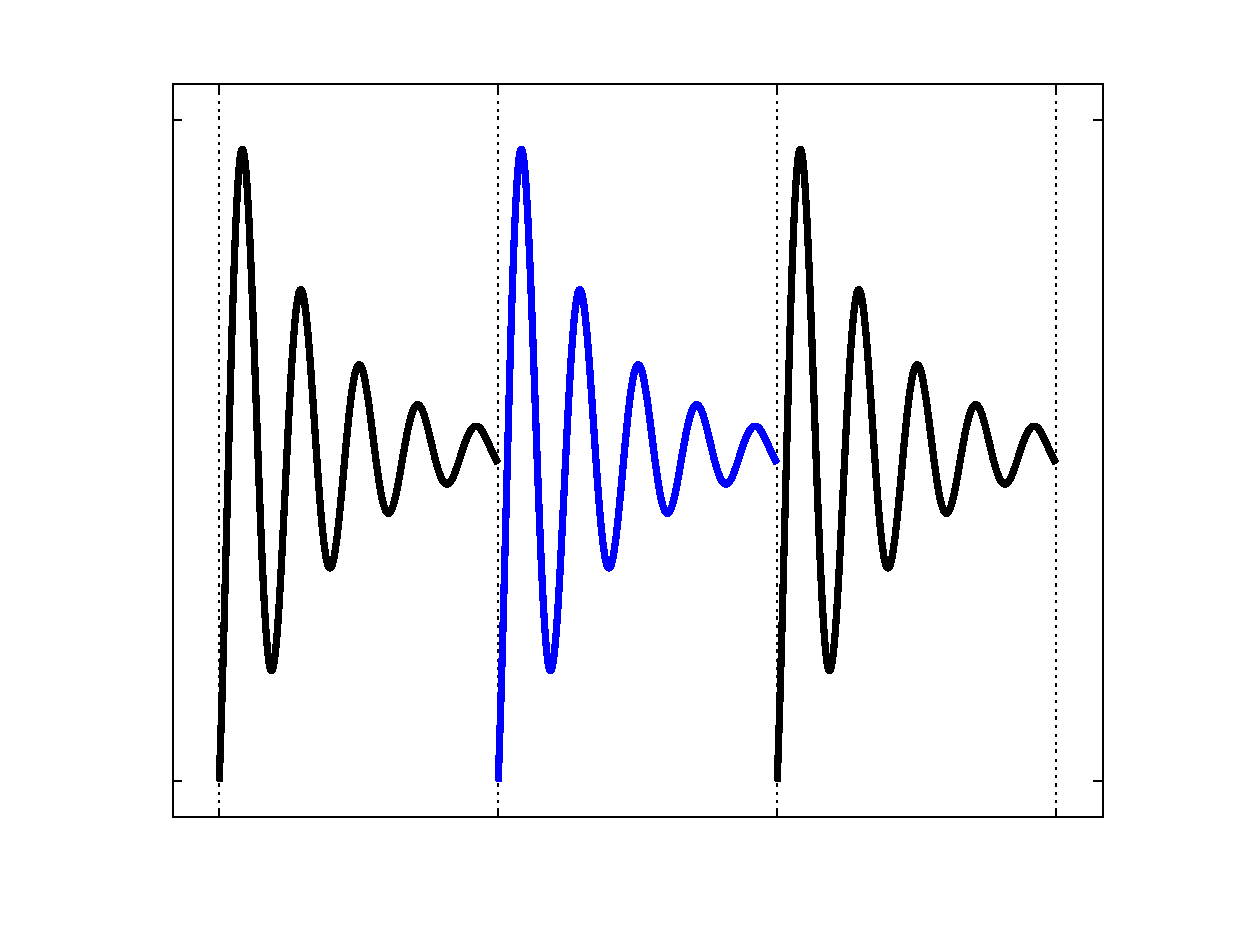
\includegraphics{FuncionPeriodica-inc}
\end{picture}%
\begin{picture}(576,432)(0,0)
\fontsize{30}{0}
\selectfont\put(97.2002,42.519){\makebox(0,0)[t]{\textcolor[rgb]{0,0,0}{{-$T$}}}}
\fontsize{30}{0}
\selectfont\put(231.12,42.519){\makebox(0,0)[t]{\textcolor[rgb]{0,0,0}{{0}}}}
\fontsize{30}{0}
\selectfont\put(365.04,42.519){\makebox(0,0)[t]{\textcolor[rgb]{0,0,0}{{T}}}}
\fontsize{30}{0}
\selectfont\put(498.96,42.519){\makebox(0,0)[t]{\textcolor[rgb]{0,0,0}{{2$T$}}}}
\end{picture}
}
    \vspace{-10pt}
    \caption{Una funcion periódica}
    \label{fig:FuncionPeriodica}
\end{figurebox}
\end{figure}

Es claro que si $T$ es un período, entonces $2T$ es otro período, ya que:
\[
f(x+2T) = f((x+T)+T) = f(x+T) = f(x)\qquad \forall x\in \mathbb{R},
\]
y si repetimos el argumento, es fácil ver que
\begin{equation}
  \label{eq:MultiploPeriodo}
  f(x+nT) = f(x) \qquad \forall x\in\mathbb{R},\quad n\in\mathbb{N}.
\end{equation}
También nos interesará saber como estrechar o estirar la gráfica de una función para acortar o alargar su período. En este sentido, es importante la siguiente propiedad. Si $f(x)$ es una función de período $T$ y $a>0$, podemos definir $g(x) = f(ax)$, que tendrá período $T' = T/a$. En efecto:
\begin{equation}
  \label{eq:EstirarPeriodo}
  g(x+T/a) = f(a(x+T/a)) = f(ax + T) = f(ax) = g(x) \qquad \forall x\in \mathbb{R} .
\end{equation}
Por último, es interesante notar que podemos sumar funciones de período común para obtener otra función periódica. Es decir, si $f(x)$ y $g(x)$ tienen periodo $T$, entonces $h = f+g$ tiene el mismo período. En efecto:
\begin{equation}
  \label{eq:SumaPeriodicas}
  h(x+T) = f(x+T) + g(x+T) = f(x) + g(x) = h(x).
\end{equation}

Como veremos, combinaremos con frecuencia las propiedades anteriores cuando tratemos con armónicos.



\subsection{Armónicos}
Los armónicos son un tipo de funciones periódicas, pero son tan importantes que podemos decir que constituyen los bloques elementales del análisis de Fourier.
\begin{mybox}
\textbf{Definición.} Llamamos \textbf{armónico} a toda función de la forma:
\begin{itemize}
  \item $A\cdot \cos(\omega x + \phi)$
  \item $A\cdot \sin(\omega x + \phi)$
\end{itemize}
En cualquier caso, diremos que $A$ es la \textbf{amplitud}, $\omega$ es la \textbf{frecuencia angular} y $\phi$ es la \textbf{fase}.
\end{mybox}

Es conocido que las funciones $\cos x$ y $\sin x$ tienen período fundamental $2\pi$, de modo que según \eqref{eq:EstirarPeriodo} un armónico de frecuencia angular $\omega$ tendrá período $\frac{2\pi}{\omega}$.

 En la práctica, junto a los armónicos nos aparecerán funciones constantes. Por tanto, en un abuso de notación, nos referiremos también a ellas como un caso particular de armónicos. Además estaremos interesados en trabajar con sucesiones de armónicos. Un ejemplo típico sería:
\[
\sin(x),\ \sin(2x),\ \sin(3x),\ \ldots,\ \sin(kx),\ \ldots .
\]
En esta sucesión, los períodos fundamentales son
\[
2\pi,\ 2\pi/2,\ 2\pi/3,\ \ldots,\ 2\pi/k,\ \ldots .
\]
Y según lo precisado anteriormente (ver \eqref{eq:MultiploPeriodo}), podemos decir que todos los términos de la sucesión tienen período $2\pi$. En general, podemos conseguir armónicos de período $2T$ cambiando la frecuencia angular (ver \eqref{eq:EstirarPeriodo}). Así, otra sucesión típica podría ser:
\[1,\ \cos\left(\frac{ \pi}{T}x\right),\ \cos\left(\frac{2 \pi}{T}x\right),\ \cos\left(\frac{3 \pi}{T}x\right),\ \ldots,\ \cos\left(\frac{k \pi}{T}x\right),\ \ldots\].
De todos modos, podemos simplificar la notación escribiendo simplemente
\[
\sin(\omega_k x)\qquad \text{o}\qquad \cos(\omega_kx),
\]
para denotar al $k$-ésimo elemento de la sucesión. Por supuesto, la frecuencia $\omega_k$ debe quedar clara según el contexto.

\section{Series de Fourier}\label{s:s2}
En esta sección vamos a estudiar un \textit{teorema de representación}. ¿Qué significa esto? Quiere decir que vamos a considerar funciones que se pueden representar de una forma especial. En particular, nos interesarán funciones que son sumas infinitas de senos y cosenos, es decir, sumas de armónicos.



\subsection{Un ejemplo sencillo}
Vamos a comenzar dando una pequeña idea de la clase de problemas que podremos abordar más tarde. Sea $f:\mathbb{R}\longrightarrow\mathbb{R}$ la función dada por:
\[
f(x) = 10\cos (x) + \sin (20x).
\]
Según lo explicado anteriormente, está claro que esta función (cuya representación gráfica podemos observar en la Figura \ref{fig:FuncionEjemplo}) es suma de armónicos con períodos fundamentales $2\pi$ y $2\pi/ 20$ , de modo que podemos decir que tanto los dos armónicos como la función $f(x)$ tienen período $2\pi$.

\begin{figure}[h]
\begin{figurebox}
    \vspace{-5pt}
    \centering
         \scalebox{0.4}{ % Title: glps_renderer figure
% Creator: GL2PS 1.3.8, (C) 1999-2012 C. Geuzaine
% For: Octave
% CreationDate: Thu Jun 26 11:04:32 2014
\setlength{\unitlength}{1pt}
\begin{picture}(0,0)
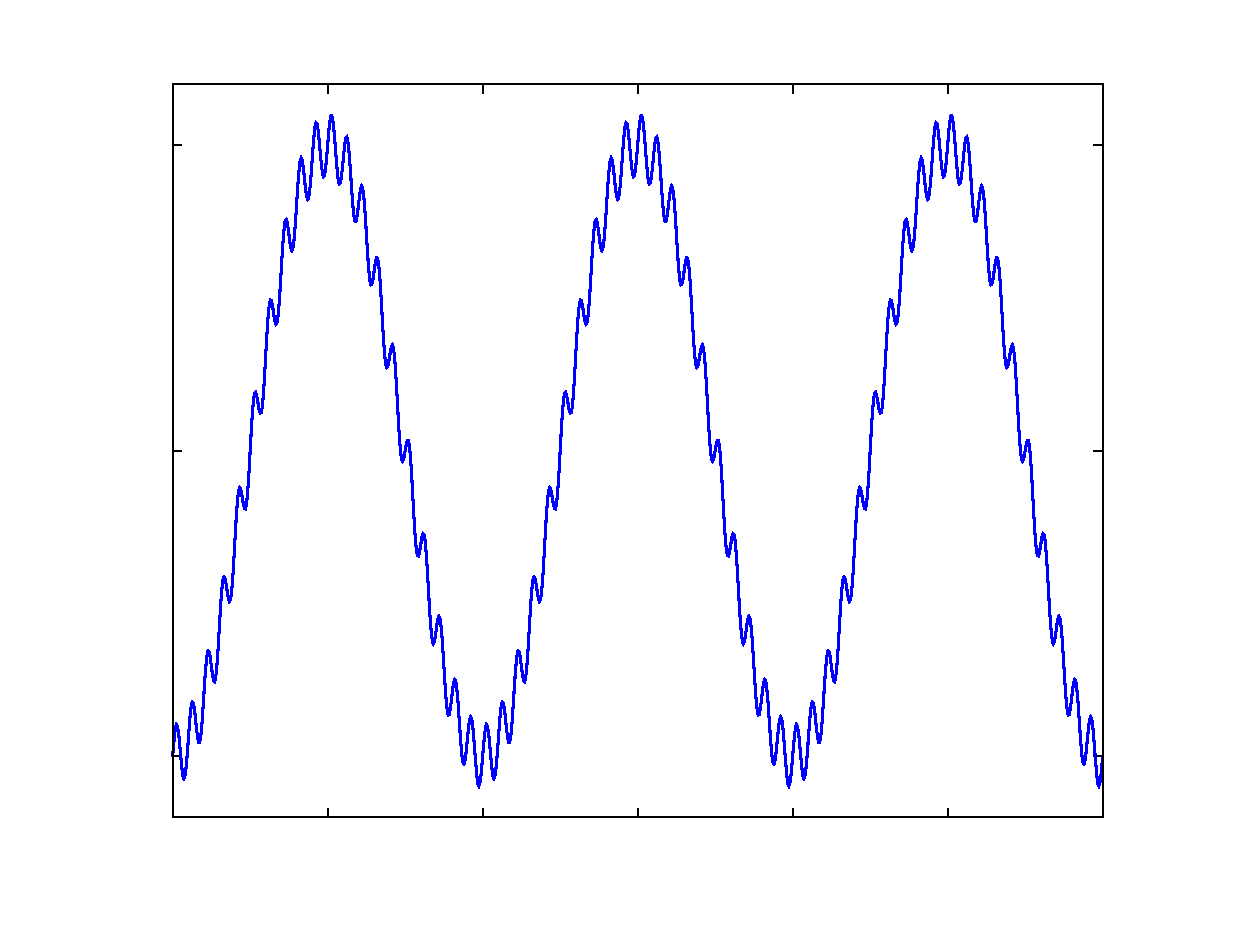
\includegraphics{FuncionEjemplo-inc}
\end{picture}%
\begin{picture}(576,432)(0,0)
\fontsize{30}{0}
\selectfont\put(149.28,42.519){\makebox(0,0)[t]{\textcolor[rgb]{0,0,0}{{-2$\pi$}}}}
\fontsize{30}{0}
\selectfont\put(223.68,34.5){\makebox(0,0)[t]{\textcolor[rgb]{0,0,0}{{-$\pi$}}}}
\fontsize{30}{0}
\selectfont\put(298.08,42.519){\makebox(0,0)[t]{\textcolor[rgb]{0,0,0}{{0}}}}
\fontsize{30}{0}
\selectfont\put(372.48,34.5){\makebox(0,0)[t]{\textcolor[rgb]{0,0,0}{{$\pi$}}}}
\fontsize{30}{0}
\selectfont\put(446.88,42.519){\makebox(0,0)[t]{\textcolor[rgb]{0,0,0}{{2$\pi$}}}}
\fontsize{30}{0}
\selectfont\put(69.8755,76.8599){\makebox(0,0)[r]{\textcolor[rgb]{0,0,0}{{-10}}}}
\fontsize{30}{0}
\selectfont\put(69.8755,223.56){\makebox(0,0)[r]{\textcolor[rgb]{0,0,0}{{0}}}}
\fontsize{30}{0}
\selectfont\put(69.8755,370.26){\makebox(0,0)[r]{\textcolor[rgb]{0,0,0}{{10}}}}
\end{picture}
}
    \vspace{-10pt}
    \caption{Suma de dos armónicos}
    \label{fig:FuncionEjemplo}
\end{figurebox}
\end{figure}

Podríamos decir que $f(x)$ es una señal con un pequeño nivel de ruido. Desde un punto de vista práctico, es útil poder eliminar el ruido para quedarnos con la parte de señal que nos interesa. Una forma de hacerlo sería transformar la función haciéndola pasar por un \textit{filtro} que elimine las frecuencias no deseadas.


\subsection{Teorema de Fourier}
En el año 1807, Joseph Fourier publicó su trabajo sobre la propagación del calor. Hasta entonces el problema sólo se sabía resolver cuando la fuente de calor se comportaba de manera sencilla (como un armónico), en cuyo caso las soluciones se llamaban funciones propias. La idea de Fourier fue descomponer una excitación cualquiera como una superposición de armónicos, de modo que la solución es la correspondiente superposición de funciones propias.

El teorema que sigue a continuación nos da las condiciones en las cuáles es lícito suponer que podemos descomponer una función como suma de otras más simples, armónicos en este caso.

\begin{mybox}

\textbf{Teorema de Fourier (caso particular).} Sea $f:\mathbb{R}\rightarrow \mathbb{R}$ una función derivable a trozos de período $2\pi$. Entonces existe una suma de armónicos que coincide con $f(x)$ en aquellos puntos en los que $f$ es continua. Más explícitamente:

Existen unos únicos coeficientes  $(a_k)$ y $(b_k)$ tales que:
  \begin{equation} \label{eq:RepresentacionFourier}
    f(x) = a_0 + \sum_{k=1}^\infty [a_k\cdot \cos(k\cdot x) + b_k\cdot \sin(k\cdot x)],
  \end{equation}
salvo en los puntos de discontinuidad.
\end{mybox}
Si $x$ es un punto en el que $f$ no es continua, la ecuacion \eqref{eq:RepresentacionFourier} podría no ser cierta. De hecho, en este caso, la suma de armónicos vale precisamente
\[
\frac{f(x^-) + f(x^+)}{2},
\]
donde $f(x^-)$ y $f(x^+)$ denotan los límites de $f$ en $x$ por la izquierda y la derecha respectivamente.
Por ejemplo, podemos considerar la señal cuadrada de la Figura \ref{fig:SignalCuadrada}:
\begin{figure}[h]
\begin{figurebox}
    \vspace{5pt}
    \centering
    \scalebox{0.4}{ % Title: glps_renderer figure
% Creator: GL2PS 1.3.8, (C) 1999-2012 C. Geuzaine
% For: Octave
% CreationDate: Thu Jun 26 11:33:43 2014
\setlength{\unitlength}{1pt}
\begin{picture}(0,0)
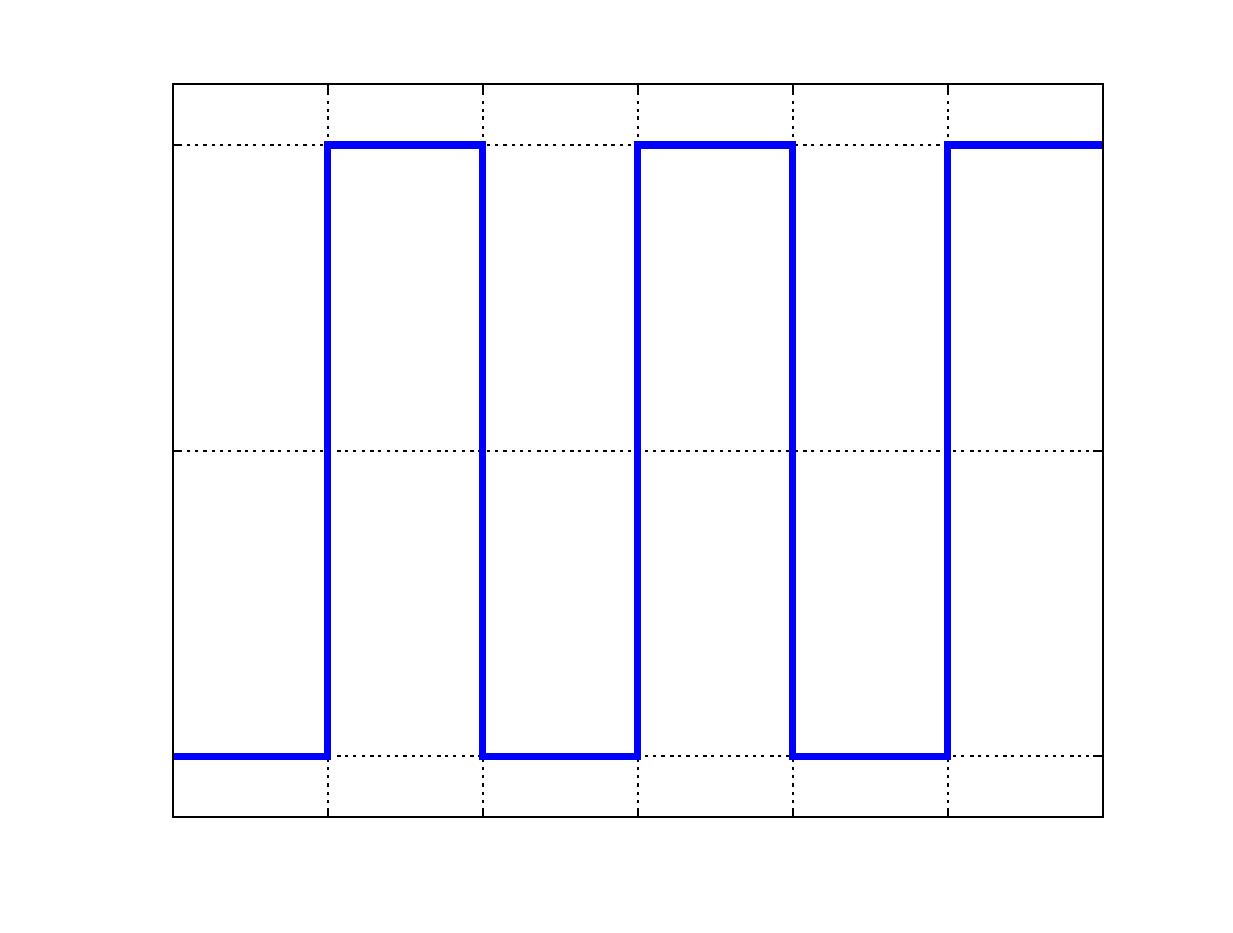
\includegraphics{Cuadrada-inc}
\end{picture}%
\begin{picture}(576,432)(0,0)
\fontsize{30}{0}
\selectfont\put(149.28,42.519){\makebox(0,0)[t]{\textcolor[rgb]{0,0,0}{{-2$\pi$}}}}
\fontsize{30}{0}
\selectfont\put(223.68,34.5){\makebox(0,0)[t]{\textcolor[rgb]{0,0,0}{{-$\pi$}}}}
\fontsize{30}{0}
\selectfont\put(298.08,42.519){\makebox(0,0)[t]{\textcolor[rgb]{0,0,0}{{0}}}}
\fontsize{30}{0}
\selectfont\put(372.48,34.5){\makebox(0,0)[t]{\textcolor[rgb]{0,0,0}{{$\pi$}}}}
\fontsize{30}{0}
\selectfont\put(446.88,42.519){\makebox(0,0)[t]{\textcolor[rgb]{0,0,0}{{2$\pi$}}}}
\fontsize{30}{0}
\selectfont\put(69.8755,76.8599){\makebox(0,0)[r]{\textcolor[rgb]{0,0,0}{{-1}}}}
\fontsize{30}{0}
\selectfont\put(69.8755,223.56){\makebox(0,0)[r]{\textcolor[rgb]{0,0,0}{{0}}}}
\fontsize{30}{0}
\selectfont\put(69.8755,370.26){\makebox(0,0)[r]{\textcolor[rgb]{0,0,0}{{1}}}}
\end{picture}
}
    \vspace{-10pt}
    \caption{Una señal cuadrada}
    \label{fig:SignalCuadrada}
\end{figurebox}
\end{figure}

Esta señal puede ser modelada por la función:
\begin{equation}
  \label{eq:SignalCuadrada}
  f(x) = 
  \begin{cases}
    -1 & \text{si } x\in\left[k\pi,(k+1)\pi\right)\quad\text{para algún }k\in\mathbb{Z}\text{ impar}\\
    +1  & \text{si } x\in\left[k\pi,(k+1)\pi\right)\quad\text{para algún }k\in\mathbb{Z}\text{ par}.
  \end{cases}
\end{equation}

Es fácil comprobar que esta función tiene período $2\pi$. Por lo tanto, el teorema de Fourier \eqref{eq:RepresentacionFourier} nos permite escribir $f(x)$ como suma de armónicos. El único problema es saber calcular los coeficientes que aparecen en la ecuación \eqref{eq:RepresentacionFourier}, así que vamos a buscar una solución.

\subsubsection*{Cálculo de los coeficientes}
Partimos de una función $f(x)$ con período $2\pi$ que cumple todos los prerrequisitos del Teorema de representación dado antes. Así, podemos escribir:
\[
f(x) = a_0 + \sum_{k=1}^\infty a_k\cos(kx) + b_k\sin(kx),
\]
y vamos a calcular la siguiente integral:
\begin{align*}
  \int_{-\pi}^{\pi}f(x)\,\mathrm{d}x 
  &=  \int_{-\pi}^{\pi}  \left[a_0 + \sum_{k=1}^\infty a_k\cos(kx) + b_k\sin(kx)\right] \,\mathrm{d}x\\
  &= a_0 \int_{-\pi}^{\pi} \,\mathrm{d}x +  \sum_{k=1}^\infty a_k  \int_{-\pi}^{\pi} \cos(kx) \,\mathrm{d}x + \sum_{k=1}^\infty b_k  \int_{-\pi}^{\pi} \sin(kx) \,\mathrm{d}x\\
  &=  a_0 \cdot 2\pi.
\end{align*}
Donde se ha utilizado que
\[
\int_{-\pi}^{\pi} \cos(kx) = 0 = \int_{-\pi}^{\pi} \sin(kx)\qquad \forall k\in \mathbb{N},
\]
para obtener
\[
\boxed{a_0 = \frac{1}{2\pi} \int_{-\pi}^{\pi} f(x)\,\mathrm{d}x.}
\]
Con la misma idea en mente podemos hacer otras integrales para deducir el resto de coeficientes:
\[
\int_{-\pi}^{\pi}f(x) \cdot \cos(kx)\,\mathrm{d}x =\ldots = \pi a_k\qquad\text{y}\qquad  \int_{-\pi}^{\pi}f(x)\cdot  \sin(kx)\,\mathrm{d}x =\ldots = \pi b_k,
\]
de donde
\[
\boxed{a_k = \frac{1}{\pi} \int_{-\pi}^{\pi} f(x)\cdot \cos(kx)\,\mathrm{d}x} \qquad \text{y} \qquad  \boxed{b_k = \frac{1}{\pi} \int_{-\pi}^{\pi} f(x)\cdot \sin(kx)\,\mathrm{d}x.}
\]
\qed


Ahora que tenemos una fórmula para sacar los coeficientes podemos seguir con el ejemplo de la señal cuadrada. Es un ejercicio sencillo demostrar que en este caso:
\[
a_0 = a_k = 0,\qquad\qquad b_k =
\begin{cases}
  \frac{4}{\pi k}&  \text{si }k\text{ es impar}\\
  0              &  \text{si }k\text{ es par. }\\
\end{cases}
\]
De modo que la suma de armónicos que representa a \eqref{eq:SignalCuadrada} es precisamente:
\begin{equation} \label{eq:Cuadrada}
f(x) = \frac{4}{\pi}\left[\sin x + \frac{1}{3}\sin(3x) + \frac{1}{5}\sin(5x) + \frac{1}{7}\sin(7x) + \frac{1}{9}\sin(9x) + \ldots\right]
\end{equation}


A veces es complicado comprender cómo se comporta una suma infinita. Además, en la práctica sólo podemos sumar un número finito de cosas, por lo tanto es necesario comprobar que una suma finita es una buena aproximación de la función. Esta comparación la podemos observar en la Figura \ref{fig:CuadradaAproximaciones}.

\begin{figure}[h]
\begin{figurebox}
    \vspace{10pt}
    \centering
      \begin{subfigure}{.3\textwidth}
          \centering
          \scalebox{0.25}{ % Title: glps_renderer figure
% Creator: GL2PS 1.3.8, (C) 1999-2012 C. Geuzaine
% For: Octave
% CreationDate: Thu Jun 26 12:41:04 2014
\setlength{\unitlength}{1pt}
\begin{picture}(0,0)
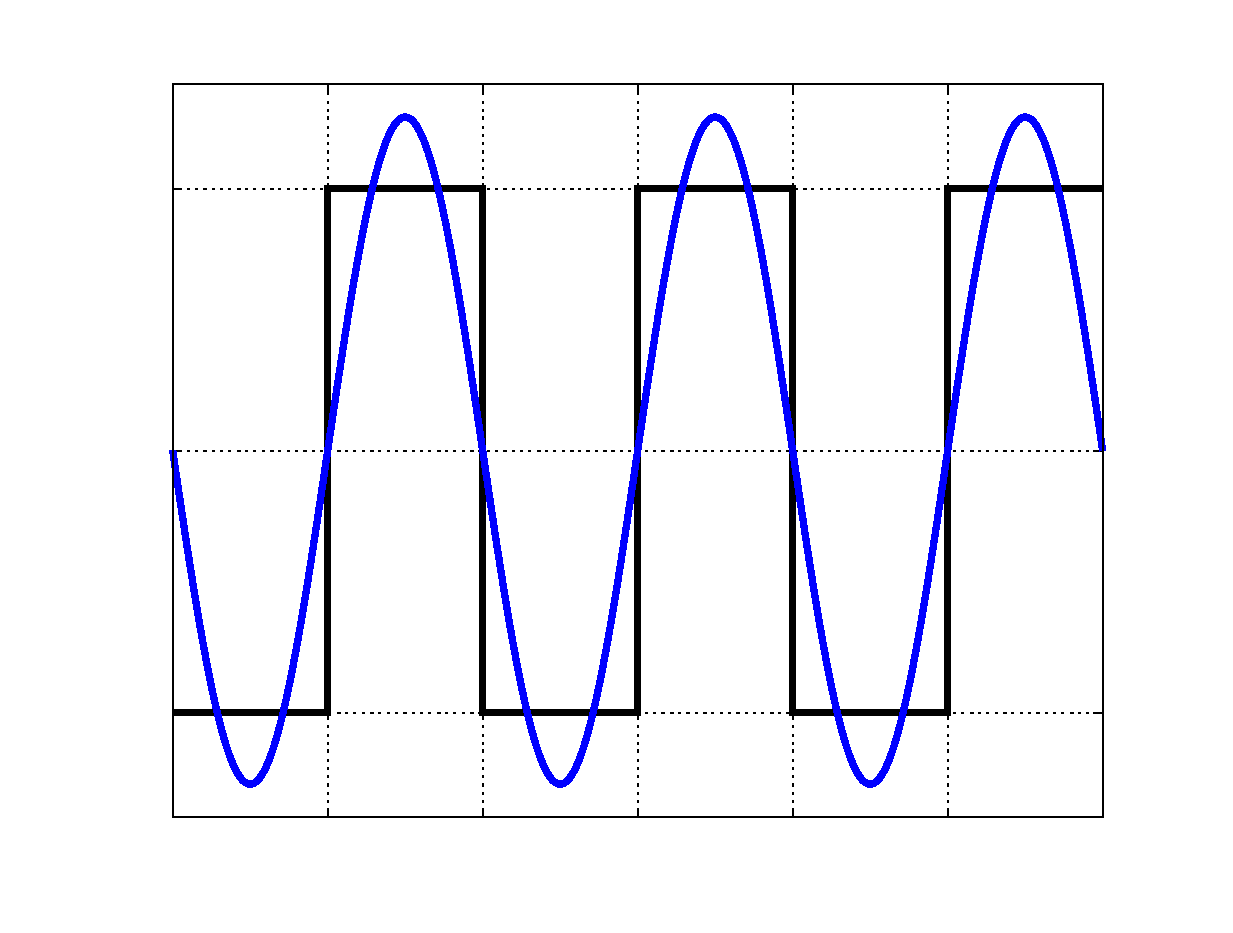
\includegraphics{CuadradaAproximaciones1-inc}
\end{picture}%
\begin{picture}(576,432)(0,0)
\fontsize{30}{0}
\selectfont\put(149.28,42.519){\makebox(0,0)[t]{\textcolor[rgb]{0,0,0}{{-2$\pi$}}}}
\fontsize{30}{0}
\selectfont\put(223.68,34.5){\makebox(0,0)[t]{\textcolor[rgb]{0,0,0}{{-$\pi$}}}}
\fontsize{30}{0}
\selectfont\put(298.08,42.519){\makebox(0,0)[t]{\textcolor[rgb]{0,0,0}{{0}}}}
\fontsize{30}{0}
\selectfont\put(372.48,34.5){\makebox(0,0)[t]{\textcolor[rgb]{0,0,0}{{$\pi$}}}}
\fontsize{30}{0}
\selectfont\put(446.88,42.519){\makebox(0,0)[t]{\textcolor[rgb]{0,0,0}{{2$\pi$}}}}
\fontsize{30}{0}
\selectfont\put(69.8755,97.8169){\makebox(0,0)[r]{\textcolor[rgb]{0,0,0}{{-1}}}}
\fontsize{30}{0}
\selectfont\put(69.8755,223.56){\makebox(0,0)[r]{\textcolor[rgb]{0,0,0}{{0}}}}
\fontsize{30}{0}
\selectfont\put(69.8755,349.303){\makebox(0,0)[r]{\textcolor[rgb]{0,0,0}{{1}}}}
\end{picture}
}
          \caption{1 armónico}
          \label{fig:0a} 
      \end{subfigure} %
      \begin{subfigure}{.3\textwidth}
          \centering
          \scalebox{0.25}{% Title: glps_renderer figure
% Creator: GL2PS 1.3.8, (C) 1999-2012 C. Geuzaine
% For: Octave
% CreationDate: Thu Jun 26 12:41:07 2014
\setlength{\unitlength}{1pt}
\begin{picture}(0,0)
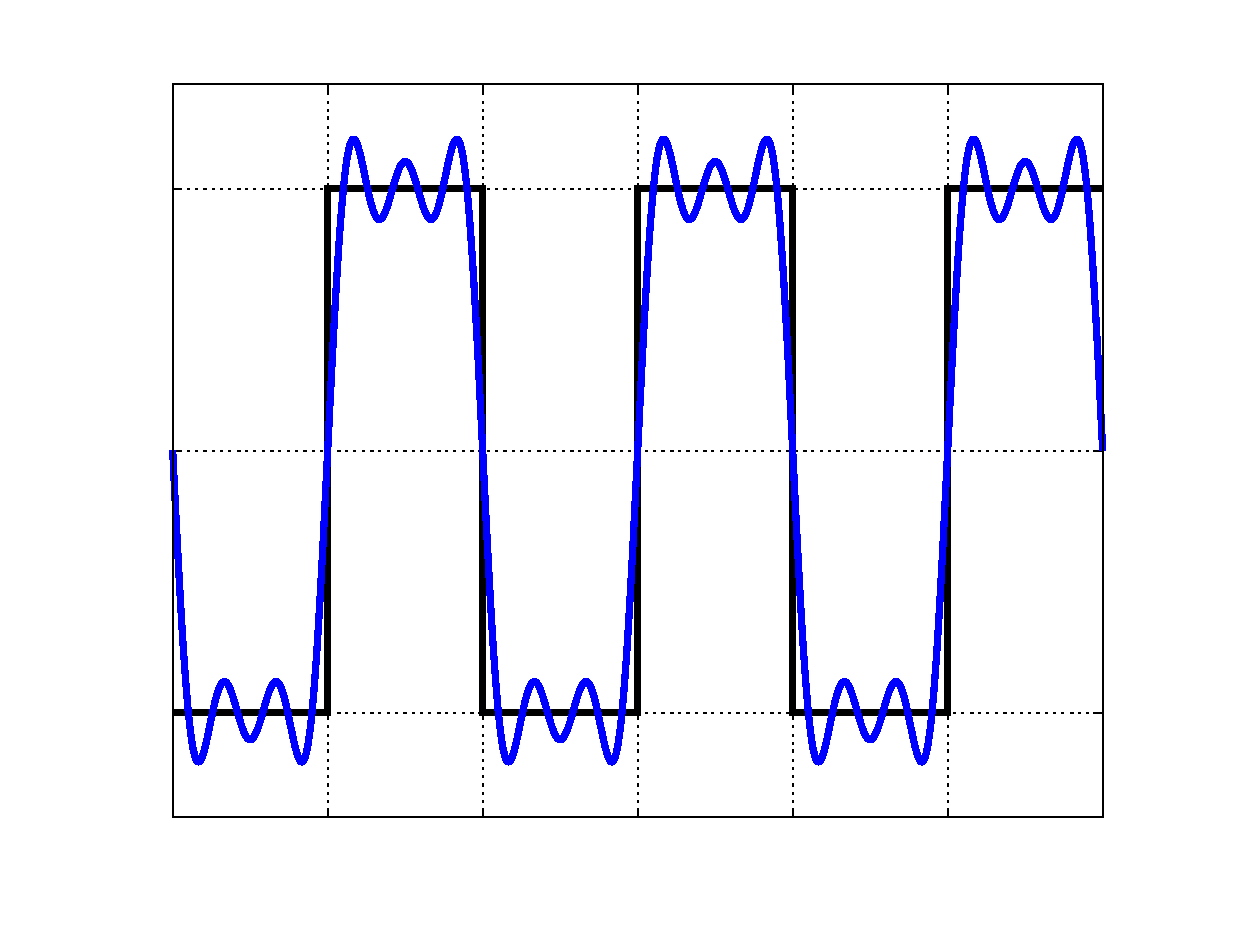
\includegraphics{CuadradaAproximaciones3-inc}
\end{picture}%
\begin{picture}(576,432)(0,0)
\fontsize{30}{0}
\selectfont\put(149.28,42.519){\makebox(0,0)[t]{\textcolor[rgb]{0,0,0}{{-2$\pi$}}}}
\fontsize{30}{0}
\selectfont\put(223.68,34.5){\makebox(0,0)[t]{\textcolor[rgb]{0,0,0}{{-$\pi$}}}}
\fontsize{30}{0}
\selectfont\put(298.08,42.519){\makebox(0,0)[t]{\textcolor[rgb]{0,0,0}{{0}}}}
\fontsize{30}{0}
\selectfont\put(372.48,34.5){\makebox(0,0)[t]{\textcolor[rgb]{0,0,0}{{$\pi$}}}}
\fontsize{30}{0}
\selectfont\put(446.88,42.519){\makebox(0,0)[t]{\textcolor[rgb]{0,0,0}{{2$\pi$}}}}
\fontsize{30}{0}
\selectfont\put(69.8755,97.8169){\makebox(0,0)[r]{\textcolor[rgb]{0,0,0}{{-1}}}}
\fontsize{30}{0}
\selectfont\put(69.8755,223.56){\makebox(0,0)[r]{\textcolor[rgb]{0,0,0}{{0}}}}
\fontsize{30}{0}
\selectfont\put(69.8755,349.303){\makebox(0,0)[r]{\textcolor[rgb]{0,0,0}{{1}}}}
\end{picture}
}
          \caption{3 armónicos}
          \label{fig:0b}
      \end{subfigure} %
      \begin{subfigure}{.3\textwidth}
          \centering
          \scalebox{0.25}{% Title: glps_renderer figure
% Creator: GL2PS 1.3.8, (C) 1999-2012 C. Geuzaine
% For: Octave
% CreationDate: Thu Jun 26 12:41:11 2014
\setlength{\unitlength}{1pt}
\begin{picture}(0,0)
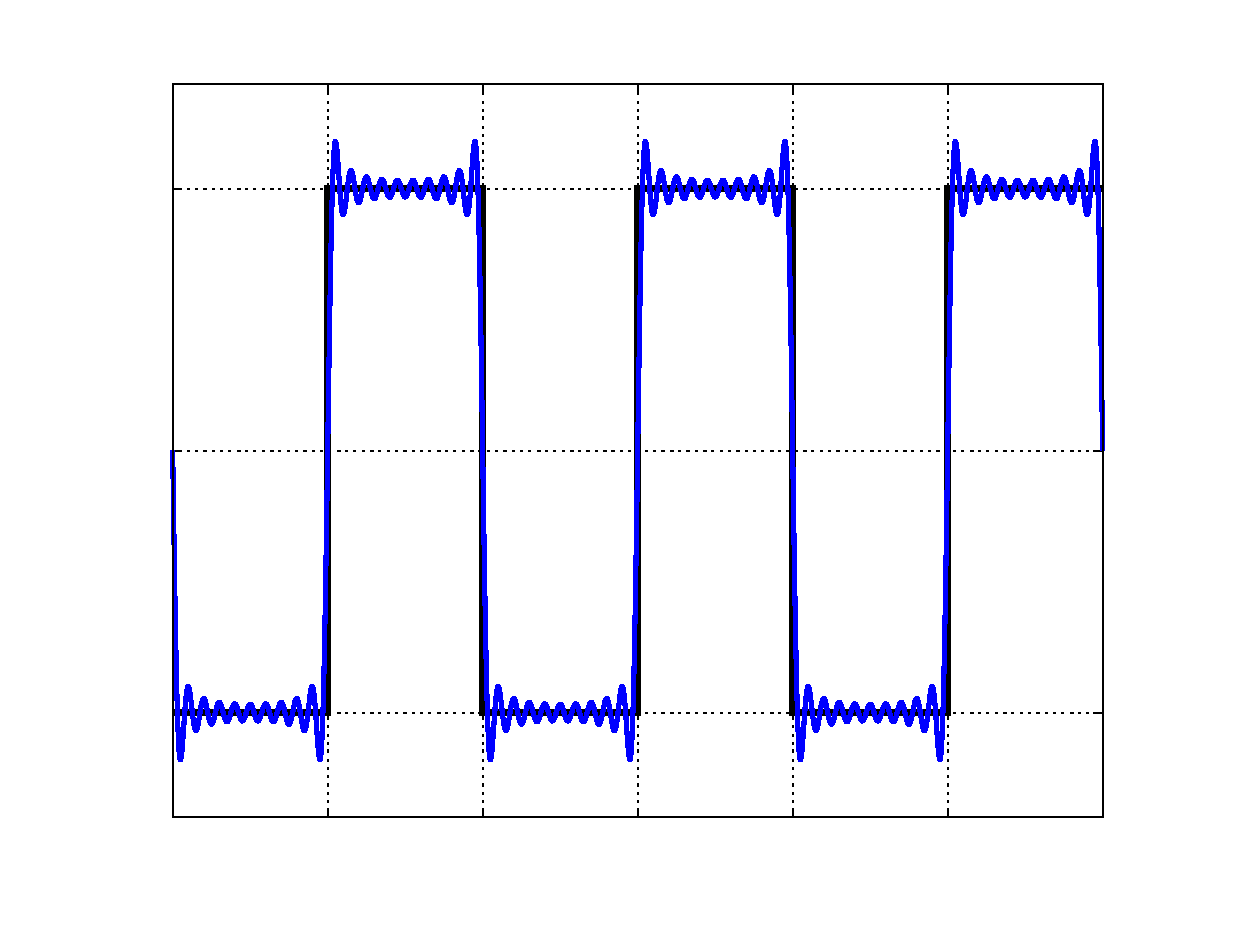
\includegraphics{CuadradaAproximaciones10-inc}
\end{picture}%
\begin{picture}(576,432)(0,0)
\fontsize{30}{0}
\selectfont\put(149.28,42.519){\makebox(0,0)[t]{\textcolor[rgb]{0,0,0}{{-2$\pi$}}}}
\fontsize{30}{0}
\selectfont\put(223.68,34.5){\makebox(0,0)[t]{\textcolor[rgb]{0,0,0}{{-$\pi$}}}}
\fontsize{30}{0}
\selectfont\put(298.08,42.519){\makebox(0,0)[t]{\textcolor[rgb]{0,0,0}{{0}}}}
\fontsize{30}{0}
\selectfont\put(372.48,34.5){\makebox(0,0)[t]{\textcolor[rgb]{0,0,0}{{$\pi$}}}}
\fontsize{30}{0}
\selectfont\put(446.88,42.519){\makebox(0,0)[t]{\textcolor[rgb]{0,0,0}{{2$\pi$}}}}
\fontsize{30}{0}
\selectfont\put(69.8755,97.8169){\makebox(0,0)[r]{\textcolor[rgb]{0,0,0}{{-1}}}}
\fontsize{30}{0}
\selectfont\put(69.8755,223.56){\makebox(0,0)[r]{\textcolor[rgb]{0,0,0}{{0}}}}
\fontsize{30}{0}
\selectfont\put(69.8755,349.303){\makebox(0,0)[r]{\textcolor[rgb]{0,0,0}{{1}}}}
\end{picture}
}
          \caption{10 armónicos}
          \label{fig:0c}
      \end{subfigure}
      % 
      \caption{Aproximación por armónicos de una señal cuadrada.}
      \label{fig:CuadradaAproximaciones}
    
\end{figurebox}
\end{figure}



Todo lo anterior se puede generalizar a funciones de período $2T$ en lugar de $2\pi$, sólo que en ese caso tendremos que estirar o encoger los armónicos para que tengan ese mismo período. 


\begin{mybox}

\textbf{Teorema de Fourier.} Sea $f:\mathbb{R}\rightarrow \mathbb{R}$ una función derivable a trozos de período $2T$. Entonces existe una suma de armónicos que coincide con $f(x)$ en aquellos puntos en los que $f$ es continua. Más explícitamente:

Existen unos únicos coeficientes  $(a_k)$ y $(b_k)$ tales que:
  \begin{equation} \label{eq:RepresentacionFourier2}
    f(x) = a_0 + \sum_{k=1}^\infty a_k\cos(\omega_kx) + b_k\sin(\omega_kx)\quad \text{ siendo }\quad \omega_k = \frac{k \pi}{T},
  \end{equation}
salvo en los puntos de discontinuidad.
\end{mybox}

El cálculo de los coeficientes cambia un poco, pero cualitativamente la situación es la misma. Un desarrollo más detallado se puede encontrar en  \cite{Asmar}.



\subsection{Una aplicación rápida}
Como ya hemos mencionado, la Figura \ref{fig:CuadradaAproximaciones} muestra que la aproximación se acerca rápido a la función\footnote{Salvo por las oscilaciones que se producen en los puntos de discontinuidad, lo que se conoce cómo \textit{fenómeno de Gibbs}.}. Vamos a pensar un poco cómo aprovechar esto.

\subsubsection*{El problema de guardar una función}
Supongamos que queremos guardar una canción en un archivo. El sonido grabado puede ser representado por una señal, que no deja de ser una función que llamaremos $f(t)$. Una solución simple sería guardar muchísimas parejas de la forma $(t, f(t))$. De hecho, deberíamos guardar infinitas parejas de esta forma para conocer la función en su totalidad. Ahora bien, como podéis imaginar, guardar infinitos valores no parece muy eficiente.

¿Qué sucede si hallamos el desarrollo de Fourier? La situación no parece cambiar mucho, ya que un conocimiento completo de la función nos exigiría guardar las infinitas parejas de coeficientes $(a_k, b_k)$. Sin embargo, la situación sí ha cambiado radicalmente. Ahora podemos decidir que nos vamos a quedar (por ejemplo) con las 100 primeras parejas de coeficientes, lo cuál es mucho más asequible.

Evidentemente, la función que reconstruyamos a partir de estos coeficientes no va a ser igual, puesto que no tenemos toda la información, pero si la serie de Fourier converge rápidamente, debería ser tremendamente parecida a la original. Dicho de otra manera, nuestro oído no será capaz de distinguir la diferencia, y a la vez estaremos ahorrando muchísimo espacio. En ideas similiares se basan los algoritmos de compresión de archivos que se utilizan en los ordenadores, como el mp3.

\begin{mybox}
  Para terminar, veamos una de las pequeñas maravillas que aparecen cuando estudiamos las series de Fourier. Si evaluamos en $x=\frac{\pi}{2}$ en la ecuación \eqref{eq:Cuadrada} y despejamos, encontramos la bonita identidad:
  \[
    \frac{\pi}{4} = 1 - \frac{1}{3} + \frac{1}{5} - \frac{1}{7} + \ldots .
  \]
\end{mybox}

\section{Enfoque complejo}\label{s:s3}
Hasta ahora hemos trabajado con números reales, combinando ingeniosamente senos y cosenos para llegar al resultado deseado. Sin embargo, resulta que los números complejos poseen ciertas peculiaridades que facilitan todos los cálculos descritos hasta ahora.

\subsection{Números complejos}
Hacemos un breve resumen (para ampliar, consultar \cite{Agarwal}). Recordemos que es común expresar un número complejo $z\in\mathbb{C}$ en forma binómica, es decir:
\[
z = a + ib,
\]
donde $i$ se conoce como unidad imaginaria (que satisface $i^2=-1$), mientras que $a$ y $b$ son números reales que reciben el nombre de parte real e imaginaria de $z$ respectivamente, lo que se suele escribir como:
\[
\operatorname{Re} (z) = a, \qquad \operatorname{Im} (z) = b.
\]
Un concepto que aparece con frecuencia es el conjugado de un número complejo $z=a+ib\in\mathbb{C}$, que se suele denotar como $\overline{z}\in \mathbb{C}$, y viene definido por
\begin{equation}
  \label{eq:Conjugado}
  \overline{z} = a - ib.
\end{equation}
Lo siguiente que repasaremos será el análogo complejo de la función exponencial.

\subsection{Exponencial compleja}
La forma más rápida de construir este concepto es recurrir a las series de potencias. En una clara analogía con la exponencial real, podemos presentar la exponencial compleja como la función $\text{exp}:\mathbb{C}\longrightarrow \mathbb{C}$ definida por:
\begin{equation}
  \label{eq:DefinicionExponencial}
  \text{exp}(z) = 1 + z + \frac{z^2}{2!} + \frac{z^3}{3!} + \ldots = \sum_{n=0}^\infty \frac{z^n}{n!}.
\end{equation}

En la práctica es común escribir simplemente $e^z$ en lugar de $\text{exp}(z)$. Esta función tiene muchísimas propiedades interesantes. Nosotros de momento destacaremos que para cualquier pareja de números complejos $z,w\in\mathbb{C}$ se tiene:
\begin{equation}
  \label{eq:PropiedadExponencial}
  e^{z+w} = e^z e^w,
\end{equation}
así como
\begin{equation}
  \label{eq:ConjugadoExponencial}
  e^{\overline{z}} = \overline{e^z}.
\end{equation}
En particular, si consideramos un número complejo en su forma binómica podemos utilizar \eqref{eq:PropiedadExponencial}:
\[
e^z = e^{a+ib} = e^a e^{ib},
\]
y ahora se puede estudiar el desarrollo en serie de potencias \eqref{eq:DefinicionExponencial} de la exponencial que involucra a la parte imaginaria para demostrar finalmente:
\[
e^{a+ib} = e^a \left[\cos b + i\sin b\right].
\]
Aquí deberíamos empezar a ver el potencial de lo que estamos haciendo. Hemos empezado a trabajar con números complejos, y resulta que al hacer exponenciales nos encontramos con senos y cosenos. Esto significa que podemos aprovechar todo nuestro conocimiento sobre exponenciales y  utilizarlo a la hora de trabajar con armónicos.

\begin{mybox}
Como apunte histórico, si  consideramos un número que solo tiene parte imaginaria encontramos la bonita igualdad
\begin{equation}
  \label{eq:EulerFormula}
  e^{i\theta}\ = \cos\theta + i\sin\theta,
\end{equation}
conocida como \textbf{fórmula de Euler}, que en el caso particular $\theta = \pi $  nos lleva a la famosa \textbf{identidad de Euler}
\[e^{i\pi} + 1 = 0.\]
\end{mybox}


\subsection{Aplicación a las series de Fourier}
Como hemos dicho, utilizaremos las exponenciales complejas para expresar las sumas de armónicos, para lo que conviene recordar todas las relaciones entre estos dos conceptos. Por un lado tenemos la fórmula de Euler \eqref{eq:EulerFormula} y por otro:
\begin{equation}
  \label{eq:ArmonicosDesdeExponencial}
  \cos x = \frac{e^{ix} + e^{-ix}}{2}, \qquad \sin x = \frac{e^{ix} - e^{-ix}}{2i}.
\end{equation}
Por tanto, vamos a considerar una función $f:\mathbb{R}\longrightarrow\mathbb{R}$ de período $2\pi$ a la que aplicarle el teorema de Fourier. Si ahora sustituimos \eqref{eq:ArmonicosDesdeExponencial} en el $k$-ésimo término del desarrollo descrito en \eqref{eq:RepresentacionFourier} encontramos:
\[
a_k\cos(kx) + b_k\sin(kx) = a_k \frac{e^{ikx} + e^{-ikx}}{2} + b_k \frac{e^{ikx} - e^{-ikx}}{2i} = \frac{1}{2}(a_k-ib_k) e^{ikx} + \frac{1}{2}(a_k+ib_k) e^{-ikx}.
\]
Y por tanto, hemos pasado de una combinación de armónicos a una combinación de exponenciales, que podemos reescribir como:
\begin{equation}
  \label{eq:kesimoExponenciales}
  a_k\cos(kx) + b_k\sin(kx) = c_k\ e^{ikx} + c_{-k}\ e^{-ikx} \qquad \text{con}\quad c_{\pm k} = \frac{1}{2}(a_k \mp ib_k).
\end{equation}
Para ganar generalidad, claramente debemos definir $c_0=a_0$ y por fin podemos dar una formulación alternativa del desarrollo de Fourier \eqref{eq:RepresentacionFourier}:
\begin{equation}
  \label{eq:FourierComplejo}
  f(x) = \sum_{k=-\infty}^\infty c_k e^{ikx}.
\end{equation}
Para terminar de redondear el resultado, vamos a echar un vistazo a los coeficientes. Estaría genial poder tener una fórmula que no nos obligue a calcular primero los coeficientes reales y después los complejos, y en efecto, basta comprobar que
\[\boxed{
c_k = \frac{1}{2\pi} \int _{-\pi}^\pi f(x) e^{-ikx} \,\text{d}x
}\]
nos lleva directamente a los coeficientes complejos\footnote{Para ello habría que definir cuidadosamente como integrar funciones complejas, pero basta con que separemos la parte real e imaginaria usando \eqref{eq:EulerFormula} e integremos cada una por separado, siendo así el resultado inmediato.}.

En el caso en el que las funciones tengan período $2T$, tenemos un resultado similar, pero de nuevo cambian ligeramente las fórmulas para calcular los coeficientes. La formulación alternativa del teorema de Fourier en este caso es:

\begin{mybox}

\textbf{Teorema de Fourier (formulación compleja).} Sea $f:\mathbb{R}\rightarrow \mathbb{R}$ una función derivable a trozos de período $2T$. Entonces existe una suma de armónicos que coincide con $f(x)$ en aquellos puntos en los que $f$ es continua. Más explícitamente:

Existen unos únicos coeficientes  $(c_k)$ tales que:
  \begin{equation} \label{eq:RepresentacionFourier3}
    f(x) = \sum_{k=-\infty}^\infty c_ke^{i\omega_k x}\quad \text{ siendo }\quad \omega_k = \frac{k \pi}{T},
  \end{equation}
salvo en los puntos de discontinuidad.
\end{mybox}

\bibliographystyle{plain}
\bibliography{fourier1}

\newpage

%%% Local Variables: 
%%% mode: latex
%%% TeX-master: "matematicaseningenieria"
%%% End: 


